\PassOptionsToPackage{unicode=true}{hyperref} % options for packages loaded elsewhere
\PassOptionsToPackage{hyphens}{url}
%
\documentclass[]{book}
\usepackage{lmodern}
\usepackage{amssymb,amsmath}
\usepackage{ifxetex,ifluatex}
\usepackage{fixltx2e} % provides \textsubscript
\ifnum 0\ifxetex 1\fi\ifluatex 1\fi=0 % if pdftex
  \usepackage[T1]{fontenc}
  \usepackage[utf8]{inputenc}
  \usepackage{textcomp} % provides euro and other symbols
\else % if luatex or xelatex
  \usepackage{unicode-math}
  \defaultfontfeatures{Ligatures=TeX,Scale=MatchLowercase}
\fi
% use upquote if available, for straight quotes in verbatim environments
\IfFileExists{upquote.sty}{\usepackage{upquote}}{}
% use microtype if available
\IfFileExists{microtype.sty}{%
\usepackage[]{microtype}
\UseMicrotypeSet[protrusion]{basicmath} % disable protrusion for tt fonts
}{}
\IfFileExists{parskip.sty}{%
\usepackage{parskip}
}{% else
\setlength{\parindent}{0pt}
\setlength{\parskip}{6pt plus 2pt minus 1pt}
}
\usepackage{hyperref}
\hypersetup{
            pdftitle={Einführung in die mathematische Datenanalyse},
            pdfauthor={Jan Heiland},
            pdfborder={0 0 0},
            breaklinks=true}
\urlstyle{same}  % don't use monospace font for urls
\usepackage{color}
\usepackage{fancyvrb}
\newcommand{\VerbBar}{|}
\newcommand{\VERB}{\Verb[commandchars=\\\{\}]}
\DefineVerbatimEnvironment{Highlighting}{Verbatim}{commandchars=\\\{\}}
% Add ',fontsize=\small' for more characters per line
\usepackage{framed}
\definecolor{shadecolor}{RGB}{248,248,248}
\newenvironment{Shaded}{\begin{snugshade}}{\end{snugshade}}
\newcommand{\AlertTok}[1]{\textcolor[rgb]{0.94,0.16,0.16}{#1}}
\newcommand{\AnnotationTok}[1]{\textcolor[rgb]{0.56,0.35,0.01}{\textbf{\textit{#1}}}}
\newcommand{\AttributeTok}[1]{\textcolor[rgb]{0.77,0.63,0.00}{#1}}
\newcommand{\BaseNTok}[1]{\textcolor[rgb]{0.00,0.00,0.81}{#1}}
\newcommand{\BuiltInTok}[1]{#1}
\newcommand{\CharTok}[1]{\textcolor[rgb]{0.31,0.60,0.02}{#1}}
\newcommand{\CommentTok}[1]{\textcolor[rgb]{0.56,0.35,0.01}{\textit{#1}}}
\newcommand{\CommentVarTok}[1]{\textcolor[rgb]{0.56,0.35,0.01}{\textbf{\textit{#1}}}}
\newcommand{\ConstantTok}[1]{\textcolor[rgb]{0.00,0.00,0.00}{#1}}
\newcommand{\ControlFlowTok}[1]{\textcolor[rgb]{0.13,0.29,0.53}{\textbf{#1}}}
\newcommand{\DataTypeTok}[1]{\textcolor[rgb]{0.13,0.29,0.53}{#1}}
\newcommand{\DecValTok}[1]{\textcolor[rgb]{0.00,0.00,0.81}{#1}}
\newcommand{\DocumentationTok}[1]{\textcolor[rgb]{0.56,0.35,0.01}{\textbf{\textit{#1}}}}
\newcommand{\ErrorTok}[1]{\textcolor[rgb]{0.64,0.00,0.00}{\textbf{#1}}}
\newcommand{\ExtensionTok}[1]{#1}
\newcommand{\FloatTok}[1]{\textcolor[rgb]{0.00,0.00,0.81}{#1}}
\newcommand{\FunctionTok}[1]{\textcolor[rgb]{0.00,0.00,0.00}{#1}}
\newcommand{\ImportTok}[1]{#1}
\newcommand{\InformationTok}[1]{\textcolor[rgb]{0.56,0.35,0.01}{\textbf{\textit{#1}}}}
\newcommand{\KeywordTok}[1]{\textcolor[rgb]{0.13,0.29,0.53}{\textbf{#1}}}
\newcommand{\NormalTok}[1]{#1}
\newcommand{\OperatorTok}[1]{\textcolor[rgb]{0.81,0.36,0.00}{\textbf{#1}}}
\newcommand{\OtherTok}[1]{\textcolor[rgb]{0.56,0.35,0.01}{#1}}
\newcommand{\PreprocessorTok}[1]{\textcolor[rgb]{0.56,0.35,0.01}{\textit{#1}}}
\newcommand{\RegionMarkerTok}[1]{#1}
\newcommand{\SpecialCharTok}[1]{\textcolor[rgb]{0.00,0.00,0.00}{#1}}
\newcommand{\SpecialStringTok}[1]{\textcolor[rgb]{0.31,0.60,0.02}{#1}}
\newcommand{\StringTok}[1]{\textcolor[rgb]{0.31,0.60,0.02}{#1}}
\newcommand{\VariableTok}[1]{\textcolor[rgb]{0.00,0.00,0.00}{#1}}
\newcommand{\VerbatimStringTok}[1]{\textcolor[rgb]{0.31,0.60,0.02}{#1}}
\newcommand{\WarningTok}[1]{\textcolor[rgb]{0.56,0.35,0.01}{\textbf{\textit{#1}}}}
\usepackage{longtable,booktabs}
% Fix footnotes in tables (requires footnote package)
\IfFileExists{footnote.sty}{\usepackage{footnote}\makesavenoteenv{longtable}}{}
\usepackage{graphicx,grffile}
\makeatletter
\def\maxwidth{\ifdim\Gin@nat@width>\linewidth\linewidth\else\Gin@nat@width\fi}
\def\maxheight{\ifdim\Gin@nat@height>\textheight\textheight\else\Gin@nat@height\fi}
\makeatother
% Scale images if necessary, so that they will not overflow the page
% margins by default, and it is still possible to overwrite the defaults
% using explicit options in \includegraphics[width, height, ...]{}
\setkeys{Gin}{width=\maxwidth,height=\maxheight,keepaspectratio}
\setlength{\emergencystretch}{3em}  % prevent overfull lines
\providecommand{\tightlist}{%
  \setlength{\itemsep}{0pt}\setlength{\parskip}{0pt}}
\setcounter{secnumdepth}{5}
% Redefines (sub)paragraphs to behave more like sections
\ifx\paragraph\undefined\else
\let\oldparagraph\paragraph
\renewcommand{\paragraph}[1]{\oldparagraph{#1}\mbox{}}
\fi
\ifx\subparagraph\undefined\else
\let\oldsubparagraph\subparagraph
\renewcommand{\subparagraph}[1]{\oldsubparagraph{#1}\mbox{}}
\fi

% set default figure placement to htbp
\makeatletter
\def\fps@figure{htbp}
\makeatother

\usepackage[]{natbib}
\bibliographystyle{plainnat}

\title{Einführung in die mathematische Datenanalyse}
\providecommand{\subtitle}[1]{}
\subtitle{Vorlesung 1}
\author{Jan Heiland}
\providecommand{\institute}[1]{}
\institute{FAU Erlangen-Nürnberg}
\date{\texttt{r\ Sys.Date()}}

\begin{document}
\maketitle

{
\setcounter{tocdepth}{1}
\tableofcontents
}
\hypertarget{vorwort}{%
\chapter*{Vorwort}\label{vorwort}}
\addcontentsline{toc}{chapter}{Vorwort}

Das ist ein Aufschrieb.

Korrekturen und Wünsche immer gerne als \emph{issues} oder \emph{pull requests} ans \href{https://github.com/highlando/script-emds}{github-repo}.

\hypertarget{was-ist-data-science}{%
\chapter{Was ist Data Science?}\label{was-ist-data-science}}

Data Science umfasst unter anderem folgende Aufgaben:

\begin{enumerate}
\def\labelenumi{\arabic{enumi}.}
\item
  Strukturieren/Aufbereiten (Umgehen mit falschen, korrumpierten, fehlenden,
  unformatierten Daten)
\item
  Data Exploration (Daten ``verstehen'')
\item
  Data Analysis (quantitative Analysen, Hypothesen aufstellen)
\item
  Data Visualization (Hypothesen graphisch kommunizieren)
\item
  Modelle erzeugen/validieren (Regeln/Muster erkennen, Vorhersagen treffen) -- \emph{das} ist Machine Learning aber es gibt auch viele andere Ansätze.
\item
  Daten Reduktion
\end{enumerate}

\hypertarget{wie-passiert-die-datenanalyse}{%
\section{Wie passiert die Datenanalyse?}\label{wie-passiert-die-datenanalyse}}

Mit mathematischen Methoden aus den Bereichen der

\begin{itemize}
\tightlist
\item
  linearen Algebra (z.B. Matrizen, Basen, lineare Gleichungssysteme)
\item
  Statistik (z.B. Mittelwerte, Korrelationen, Verteilungen)
\item
  Analysis (Grenzwerte, Abschätzungen)
\item
  \ldots{}
\end{itemize}

Dabei hilft Software, z.B.,

\begin{itemize}
\tightlist
\item
  Excel
\item
  \textbf{Python}
\item
  Matlab
\item
  R
\end{itemize}

bei der Berechnung, Automatisierung, Visualisierung.

\begin{quote}
Python ist ein de-facto Standard in Data Science und Machine Learning.
\end{quote}

\hypertarget{was-sind-daten}{%
\section{Was sind Daten?}\label{was-sind-daten}}

Wie sehen Daten aus?

\begin{itemize}
\item
  Numerisch reell, z.B. Temperatur
\item
  Numerisch diskret, z.B. Anzahl
\item
  Ordinal: Element einer festen Menge mit expliziter Ordnung, z.B.
  \{neuwertig, mit Gebrauchsspuren, defekt\}
\item
  Binär: Eine von zwei Möglichkeiten, z.B. Wahr/Falsch oder aktiv/inaktiv
\item
  Kategoriell: Element einer festen Menge ohne klare Ordnung, z.B.
  \{Säugetier, Vogel, Fisch\}
\item
  sonstige strukturierte Daten, z.B. geographische Daten, Graphen
\item
  reiner Text, z.B. Freitext in Restaurantbewertung
\end{itemize}

Und allgemeine Eigenschaften. Sind die Daten

\begin{itemize}
\tightlist
\item
  strukturiert
\item
  lückenhaft
\item
  fehlerbehaftet (\emph{verrauscht})
\item
  interpretierbar
\item
  geordnet (oder nicht zu ordnen)
\end{itemize}

\hypertarget{beispiele}{%
\section{Beispiele}\label{beispiele}}

\hypertarget{tabellendaten-mietpreise}{%
\subsection{Tabellendaten -- Mietpreise}\label{tabellendaten-mietpreise}}

\begin{figure}
\centering
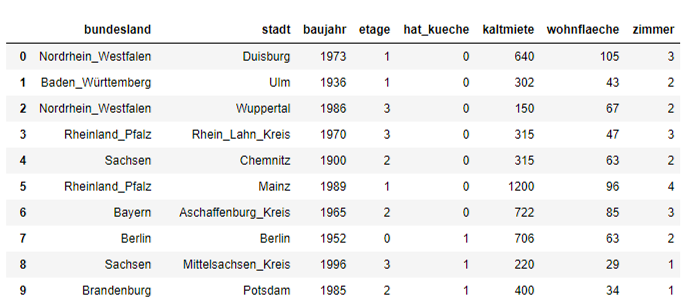
\includegraphics{bilder/dataframe.png}
\caption{image}
\end{figure}

Hier wären die Aufgaben von Data Science:

\begin{itemize}
\tightlist
\item
  Daten ``verstehen'', Zusammenhänge zwischen
  Variablen aufdecken,
\item
  visualisieren.
\item
  Gegebenenfalls fehlende Einträge bei (z.B.) \texttt{kaltmiete} vorhersagen
\end{itemize}

\begin{figure}
\centering
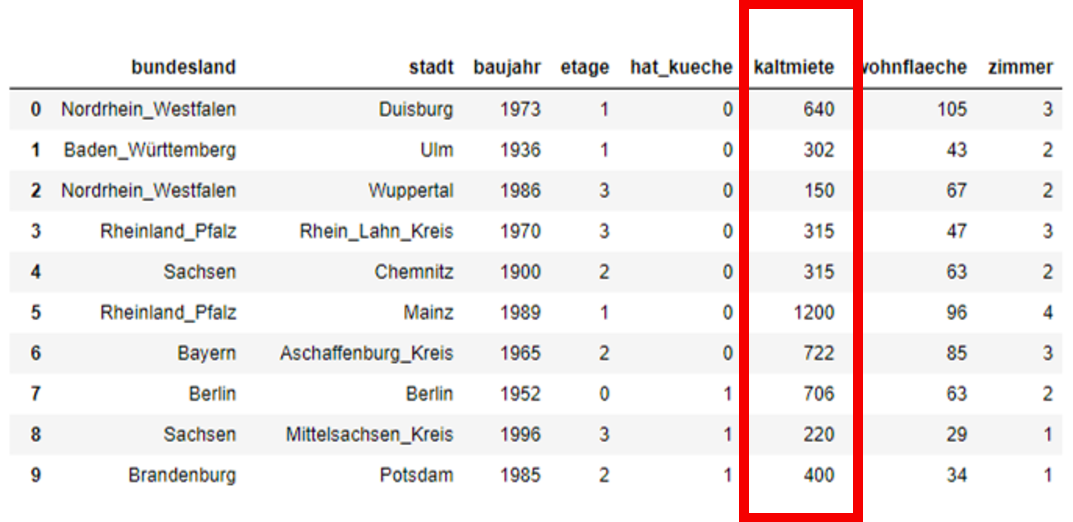
\includegraphics{bilder/dataframe_spalte.pdf}
\caption{image}
\end{figure}

Datenexploration und -analyse für einzelne Variablen 1/3 Wir betrachten
eine \emph{numerische} Variable in einem rechteckigen Datensatz, also eine
\emph{Spalte} (z.B. \texttt{kaltmiete}). Wir bezeichnen den \(i\)-ten Eintrag in
dieser Spalte mit \(x_i\), wobei \(i=1,\ldots,N\) (\(N\) Anzahl der Zeilen).

Folgende \emph{Schätzer}/\emph{Metriken} können dabei helfen, diese Spalte besser
zu verstehen:

\begin{itemize}
\item
  Mittelwert \(\overline x= \frac1 N\sum_{i=1}^N x_i\)
\item
  gewichteter Mittelwert
  \(\overline x_w = \frac{\sum_{i=1}^N w_i x_i}{\sum_{j=1}^N w_j}\),
  wobei \(w_i\) das Gewicht des \(i\)-ten Eintrages ist (z.B. eine andere
  Variable).
\item
  Varianz: \(s_x^2 = \frac{1}{N-1} \sum_{i=1}^N (x_i-\overline x)^2\)
\item
  Standardabweichung \(s = \sqrt{s_x^2}\).
\item
  Median = \(\frac{315 + 400}{2} = 357.5\).
\end{itemize}

Datenexploration und -analyse für mehrere Variablen Wir betrachten zwei
Spalten \(x = (x_1,\ldots,x_N)\) und \(y = (y_1,\ldots, y_N)\).\\

\textbf{Scatter Plot}

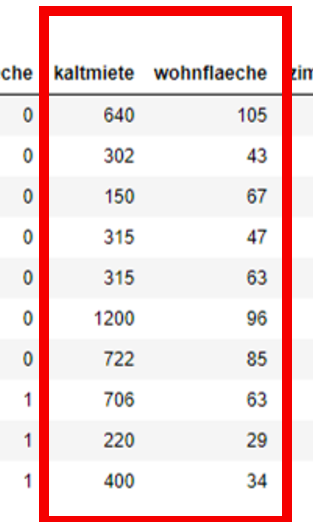
\includegraphics[width=0.27\textwidth,height=\textheight]{bilder/dataframe_spalte3.pdf}
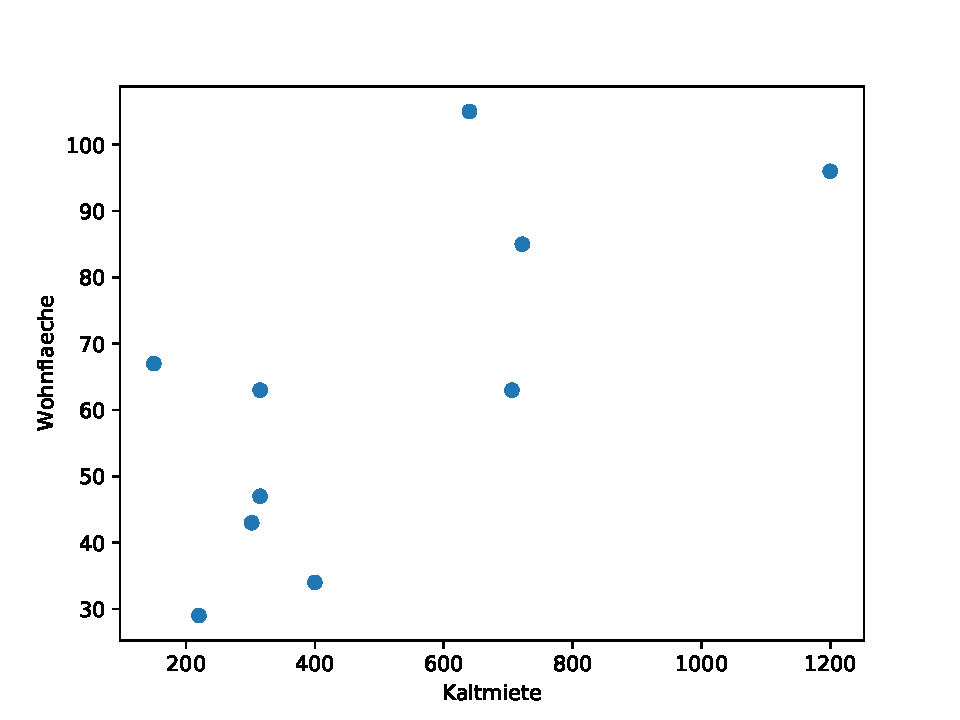
\includegraphics[width=0.7\textwidth,height=\textheight]{bilder/scatterplot.pdf}

Datenexploration und -analyse für mehrere Variablen Wir betrachten zwei
Spalten \(x = (x_1,\ldots,x_N)\) und \(y = (y_1,\ldots, y_N)\).

\begin{itemize}
\item
  Kovarianz
  \(s_{xy} = \frac{1}{N-1}\sum_{i=1}^N (x_i - \overline x)(y_i - \overline y)\)
\item
  Korrelation \(\rho_{xy} = \frac{s_{xy}}{s_x\cdot s_y} \in [-1,1]\).
\item
  \(\rho \approx 1\): Starke positive Korrelation, wenn \(x\) groß ist,
  ist \(y\) auch groß.
\item
  \(\rho \approx -1\): Starke negative Korrelation, wenn \(x\) groß ist,
  ist \(y\) klein
\item
  \(\rho \approx 0\): Wenig/keine Korrelation.
\end{itemize}

\begin{figure}
\centering
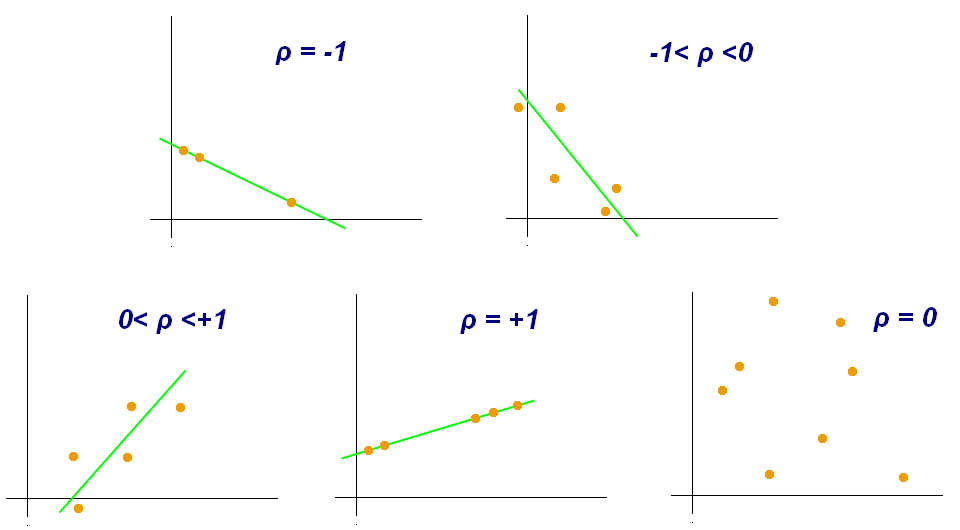
\includegraphics[width=0.65\textwidth,height=\textheight]{bilder/Correlation_coefficient.png}
\caption{Von Kiatdd - Eigenes Werk, CC BY-SA 3.0, \url{https://commons.wikimedia.org/w/index.php?curid=37108966}}
\end{figure}

\hypertarget{covid-19-daten}{%
\subsection{COVID-19 Daten}\label{covid-19-daten}}

Vergleiche die Einführung in \emph{Mathematik für Data Science 1} vom letzten Semester.

\hypertarget{netflix-prize}{%
\subsection{Netflix Prize}\label{netflix-prize}}

Hierbei geht es darum, ob aus bekannten Bewertungen von vielen verschiedenen Benutzern für viele verschiedene Filme abgeleitet werden kann, ob ein bestimmter Nutzer einen bestimmten Film mag (also positiv bewerten würde).

Vergleiche auch \href{https://en.wikipedia.org/wiki/Netflix_Prize}{Wikipedia:Netflix\_Prize}

Das (Trainings-)Daten bestehen über \texttt{480189} Benutzer, die für \texttt{17770} Filme insgesamt \texttt{100480507} Bewertungen als ganze Zahlen zwischen \texttt{1} und \texttt{5} verteilten.

Ziel der Datenanalyse war es, für \texttt{2817131} ``Paare'' von Benutzern und Filmen, die Bewertung vorauszusagen. Neben der schieren Masse an Daten kamen noch Einschränkungen hinzu, die ein Mindestmaß an Qualität der Vorhersage sicherstellen sollten.

Das Problem ließe sich wie folgt darstellen.

\begin{longtable}[]{@{}llllll@{}}
\toprule
Benutzer \textbackslash{} Film & \texttt{1} & \texttt{2} & \texttt{...} & \texttt{n} & \texttt{...}\tabularnewline
\midrule
\endhead
\texttt{1} & -- & 3 & \texttt{...} & 5 & \texttt{...}\tabularnewline
\texttt{2} & 3 & 4 & \texttt{...} & 2 & \texttt{...}\tabularnewline
\texttt{3} & 1 & 2 & \texttt{...} & \textbf{?} & \texttt{...}\tabularnewline
\texttt{...} & 3 & 4 & \texttt{...} & -- & \texttt{...}\tabularnewline
\bottomrule
\end{longtable}

Gegeben viele (aber bei weitem nicht alle) Einträge in einer riesigen Tabelle. Können wir aus den Zusammenhängen bestimmte fehlende Einträge (z.B. wie findet Nutzer \texttt{3} den Film \texttt{n}) herleiten?

Die besten Lösungen für dieses Problem basieren durchweg auf \emph{Machine Learning} Ansätzen.

\hypertarget{python}{%
\section{Python}\label{python}}

Die Programmiersprache \texttt{python} wird uns durchs Semester begleiten. Einfach weil sie so wichtig ist für \emph{Data Science} aber auch weil sie (meiner Meinung nach) einfach zu erlernen und zu benutzen ist.

\hypertarget{aufgaben}{%
\section{Aufgaben}\label{aufgaben}}

\hypertarget{a1-python}{%
\subsection{A1 -- Python}\label{a1-python}}

Bringen sie ihr \texttt{python} zum Laufen, installieren sie \texttt{numpy}, \texttt{scipy} und \texttt{matplotlib} und führen sie das folgende script aus.

\begin{Shaded}
\begin{Highlighting}[]
\ImportTok{import}\NormalTok{ numpy }\ImportTok{as}\NormalTok{ np}
\ImportTok{import}\NormalTok{ matplotlib.pyplot }\ImportTok{as}\NormalTok{ plt}

\NormalTok{N }\OperatorTok{=} \DecValTok{20}
\NormalTok{xmax }\OperatorTok{=} \DecValTok{2}
\NormalTok{xmin }\OperatorTok{=} \DecValTok{0}

\NormalTok{xdata }\OperatorTok{=}\NormalTok{ np.linspace(xmin, xmax, N)}
\NormalTok{ydata }\OperatorTok{=}\NormalTok{ np.exp(xdata)}

\NormalTok{plt.figure(}\DecValTok{1}\NormalTok{)}
\NormalTok{plt.plot(xdata, ydata, }\StringTok{'.'}\NormalTok{)}

\NormalTok{plt.figure(}\DecValTok{2}\NormalTok{)}
\NormalTok{plt.semilogy(xdata, ydata, }\StringTok{'.'}\NormalTok{)}
\NormalTok{plt.show()}
\end{Highlighting}
\end{Shaded}

\hypertarget{a2-einheitsmatrix}{%
\subsection{A2 -- Einheitsmatrix}\label{a2-einheitsmatrix}}

Schreiben sie ein script, dass die \texttt{5x5} Einheitsmatrix auf 3 verschiedene Arten erzeugt. (Eine Art könnte die eingebaute \texttt{numpy} Funktion \texttt{eye} sein).

\begin{Shaded}
\begin{Highlighting}[]
\ImportTok{import}\NormalTok{ numpy }\ImportTok{as}\NormalTok{ np}

\NormalTok{idfive }\OperatorTok{=}\NormalTok{ np.eye(}\DecValTok{5}\NormalTok{)}
\BuiltInTok{print}\NormalTok{(idfive)}
\end{Highlighting}
\end{Shaded}

Hinweis: schauen sie sich mal an wie \texttt{numpy}'s \texttt{arrays} funktionieren.

\hypertarget{matrizen-multiplikation-und-potenz}{%
\subsection{3 -- Matrizen Multiplikation und Potenz}\label{matrizen-multiplikation-und-potenz}}

Schreiben sie ein script, das die Übungsaufgabe aus der Vorlesung (potenzieren der Matrizen \(M_i\), \(i=1,2,3,4\)) löst. Zum Beispiel mit

\begin{Shaded}
\begin{Highlighting}[]
\ImportTok{import}\NormalTok{ numpy }\ImportTok{as}\NormalTok{ np}
\NormalTok{mone }\OperatorTok{=}\NormalTok{ np.array([[}\FloatTok{0.9}\NormalTok{, }\FloatTok{0.9}\NormalTok{], [}\FloatTok{0.9}\NormalTok{, }\FloatTok{0.9}\NormalTok{]])}

\NormalTok{mone_ptwo }\OperatorTok{=}\NormalTok{ mone }\OperatorTok{@}\NormalTok{ mone}
\BuiltInTok{print}\NormalTok{(mone_ptwo)}

\NormalTok{mone_pfour }\OperatorTok{=}\NormalTok{ mone_ptwo }\OperatorTok{@}\NormalTok{ mone_ptwo}
\BuiltInTok{print}\NormalTok{(mone_pfour)}
\end{Highlighting}
\end{Shaded}

Oder so:

\begin{Shaded}
\begin{Highlighting}[]
\ImportTok{import}\NormalTok{ numpy }\ImportTok{as}\NormalTok{ np}
\NormalTok{mone }\OperatorTok{=}\NormalTok{ np.array([[}\FloatTok{0.9}\NormalTok{, }\FloatTok{0.9}\NormalTok{], [}\FloatTok{0.9}\NormalTok{, }\FloatTok{0.9}\NormalTok{]])}
\NormalTok{mone_p }\OperatorTok{=}\NormalTok{ np.eye(}\DecValTok{2}\NormalTok{)}

\ControlFlowTok{for}\NormalTok{ k }\KeywordTok{in} \BuiltInTok{range}\NormalTok{(}\DecValTok{16}\NormalTok{):}
\NormalTok{    mone_p }\OperatorTok{=}\NormalTok{ mone_p }\OperatorTok{@}\NormalTok{ mone}
    \ControlFlowTok{if}\NormalTok{ k }\OperatorTok{==} \DecValTok{1} \KeywordTok{or}\NormalTok{ k }\OperatorTok{==} \DecValTok{3} \KeywordTok{or}\NormalTok{ k }\OperatorTok{==} \DecValTok{15}\NormalTok{:}
        \BuiltInTok{print}\NormalTok{(}\StringTok{'k='}\NormalTok{, k}\OperatorTok{+}\DecValTok{1}\NormalTok{)}
        \BuiltInTok{print}\NormalTok{(mone_p)}
\end{Highlighting}
\end{Shaded}

Achtung:

\begin{itemize}
\tightlist
\item
  bei Matrizen kann auch \texttt{*} benutzt werden -- das ist aber nicht die richtige Matrizenmultiplikation (sondern die Multiplikation eintragsweise)
\item
  Moegliche Realisierung der Matrizenmultiplikation

  \begin{itemize}
  \tightlist
  \item
    \texttt{np.dot(A,\ B)} -- die klassische Methode
  \item
    \texttt{A.dot(B)} -- das selbe (manchmal besser, wenn \texttt{A} etwas allgemeiner ist (zum Beispiel eine \texttt{scipy.sparse} matrix)
  \item
    \texttt{A\ @\ B} -- convenience Notation
  \end{itemize}
\end{itemize}

\end{document}
